\documentclass[15pt]{article}
\usepackage{amssymb}
\usepackage[margin=1in]{geometry}		% For setting margins
\usepackage{amsmath}				% For Math
\usepackage{fancyhdr}				% For fancy header/footer
\usepackage{graphicx}				% For including figure/image
\usepackage{float}
\usepackage{cancel}					% To use the slash to cancel out stuff in work

%%%%%%%%%%%%%%%%%%%%%%
% Set up fancy header/footer
\pagestyle{fancy}
\fancyhead[LO,L]{Arvid Kolstad - 020814-8452}
\fancyhead[RO,R]{FFR110 - Assignment 3 problem 1 }
\fancyfoot[LO,L]{}
\fancyfoot[CO,C]{\thepage}
\fancyfoot[RO,R]{}
\renewcommand{\headrulewidth}{0.4pt}
\renewcommand{\footrulewidth}{0.4pt}
%%%%%%%%%%%%%%%%%%%%%%

\begin{document}
\section{Problem 1}
In this report problem 1 for assignment 3 is going to be presented and solved. The system we are studying in this problem is the following:
\begin{equation}
	\frac{dI}{dt} = \frac{\alpha}{N}SI - \beta I
	\label{eq:system1}
\end{equation}
\begin{equation}
	\frac{dS}{dt} = -\frac{\alpha}{N}SI + \beta I
	\label{eq:system2}
\end{equation}
where $I$ is the number of infected people, $S$ is the number of susceptible people and $N = S+I$ is constant. The system is often called the SIS-model and describes how a disease can spread trough a population.
\subsection{a)}
In this part we are supposed to argue at which values for the deterministic SIS-model that the number of susceptible and infected stays constant with time. We therefore start with finding the steady states for the model trough a linear analysis. The start by rewriting the system as the following:
\begin{equation}
	\frac{dI}{dt} = \frac{\alpha}{N}(N-I)I - \beta I = 0
	\label{eq:1d system}
\end{equation}
to get the 1D representation of the system. If we solve for the steady states for this system we get all the steady states for the whole system is $I^*_1 = 0$ which gives us $S^*_1 = N$. If we then look at the case where $I \neq 0$ we have to following:
\begin{equation}
	\frac{dI}{dt} = \frac{\alpha}{N}(N-I) - \beta  = 0
\end{equation}
If we solve this for I we get the following:
\begin{equation}
	I^*_2 = N(1-\frac{\beta}{\alpha}) = N(1- \frac{1}{r_0} \implies S^*_2  = N\frac{\beta}{\alpha}
	\label{eq:I_2^*}
\end{equation}
We now do the linear analysis of the system and get the following:
\begin{equation}
	\frac{d^2I}{dIdt} = \frac{\alpha}{N}(N-2I) - \beta
	\label{eq:dI/dI}
\end{equation}
If we take $I_1^*$ and substitute in equation \ref{eq:dI/dI} we get the following:
\begin{equation}
	\frac{\alpha}{N}(N) - \beta = \alpha - \beta
	\label{eq:StabilityI1}
\end{equation}
If we take $I_2^*$ and substitute in equation \ref{eq:dI/dI} we get the following:
\begin{equation}
	\frac{\alpha}{N}(N-2N(1 - \frac{\beta}{\alpha})) - \beta = \beta - \alpha
	\label{eq:StabilityI2}
\end{equation}
With these results we can know say that $N^*_2$ will be stable if $r_0 > 1$ and otherwise unstable and $N_1^*$ will be stable if $r_0 < 0$ and otherwise unstable. Therefore we can say that $N^*_2$ will be attracting and sustained if at infinite times if $r_0 > 1$ and otherwise will $N^*_1$ be attracting and sustaining.
\subsection{b)}
In this part we will show how the deterministic model of the SIS-model will be derived of the stochastic version of the model when $N \rightarrow \infty$. To start this we write the stochastic version of the SIS-model:
\begin{equation}
	\begin{cases}
		n \rightarrow n+1, & \text{at rate }b_n = \alpha n (1- \frac{1}{r_0}) \\
		n \rightarrow n-1, & \text{at rate }d_n = \beta n                     \\
	\end{cases}
	\label{eq:stochastic equations}
\end{equation}
If we now look at a very small time step from $t \rightarrow t + \delta t$ we have the following probability function:
\begin{equation}
	\rho_n(t+ \delta t) = \rho_n(t) + \left(b_{n-1}\rho_{n-1}(t) + d_{n+1}\rho_{n+1}(t)\right)\delta t - (b_n - d_n)\rho_n(t)\delta t
\end{equation}
after some quick algebra we now got this expression:
\begin{equation}
	\frac{\rho_n(t+ \delta t) - \rho_n(t)}{\delta t}  = b_{n-1}\rho_{n-1}(t) + d_{n+1}\rho_{n+1}(t) - (b_n - d_n)\rho_n(t)
	\label{eq:}
\end{equation}
now let $\delta t \rightarrow 0$ we get the following:
\begin{equation}
	\frac{d\rho_n}{dt}= b_{n-1}\rho_{n-1}(t) + d_{n+1}\rho_{n+1}(t) - (b_n - d_n)\rho_n(t)
\end{equation}
which is the master equation. As in the lecture notes, we introduce the following notation: $ I = \frac{n}{N}$, $\lambda (I) = \alpha I (1-I)$ and $\mu (I)= \beta I$. With this notation we can now write the following expressions:
\begin{equation}
	b_n = N \alpha I(1-I) = N \lambda(I)
\end{equation}
\begin{equation}
	d_n = N \beta I = N\mu(I)
\end{equation}
We also use the notation of step operators $\mathbb{E^+}\rho_n= \rho_{n+1}$.
Rewriting the master equation with this notation we get the following:
\begin{equation}
	\frac{d\rho_n}{dt} = (\mathbb{E^-} -1) \lambda_n \rho_n + (\mathbb{E^+}- 1)\mu_n \rho_n
\end{equation}
If we now rewrite $\rho_{n \pm1}(t) = \rho(n \pm 1, t) =g(I \pm \frac{1}{N}, t)$ we can think of $\frac{1}{N}$ as just a small deviation around $I$ and if we also say that $p(I, t)$ is a smooth function we can do the the following expansion:
\begin{equation}
	\mathbb{E^\pm}g(I) = g(I \pm \frac{1}{N}) = \sum_{k=0}^{\infty} \frac{(\pm\frac{1}{N})^k}{k!} \frac{d^kg}{dI^k} = e^{\frac{1}{N}\frac{d}{dI}} g \prime (I)
\end{equation}
this transforms the master equation to the following:
\begin{equation}
	\frac{\partial\rho_n}{\partial t} = \left(e^{-\frac{1}{N}\frac{\partial}{\partial I} }-1 \right) N\lambda(I)\rho(I)+\left(e^{\frac{1}{N}\frac{\partial}{\partial I}} -1 \right) N\mu(I)\rho(I)
\end{equation}
if we now approximate this expression for small deviations from $I$ and only take the linear terms from the taylor expansion we get the following expression:
\begin{equation}
	\frac{\partial}{\partial I}(\mu(I) - \lambda(I))\rho(I)
\end{equation}
if we now call $v(I) = \lambda(I) - \mu(I)$ we get the so called transport equation:
\begin{equation}
	\frac{\partial g(I,t)}{\partial t} + \frac{\partial }{\partial I}v(I)g(I,t) = 0
\end{equation}
As we let $N \rightarrow \infty$ the probabilistic density is concentrated to one point and the system therefore follows a deterministic trajectory which have the dynamics of the form:
\begin{equation}
	\frac{dI}{dt} = v(I)
\end{equation}
Up to a scaling factor this is gives the same solutions as the deterministic system, which means that we proved what we wanted to prove.
\subsection{c)}
In this section a total of 6 distributions where supposed to be sampled to show that they could be described by an exponential distribution. The distributions that were supposed to be sampled was the probability of the time to the next infection occurring and the time to the next recovery occurring where equation \ref{eq:stochastic equations} is ruling. Therefore was the recovery and infection distribution sampled in pairs. Down below the 3 samplings that where ran can be found. For every distribution 5000 samples where collected.

\begin{figure}[H]
	\begin{center}
		
\includegraphics[width=0.95\textwidth]{figures/distribution_plot1.pdf}
	\end{center}
	\caption{In the left plot we can see the distribution for the infection time with a $b_n = 0.1$. We see that the fitted exponential distribution fits very well where we get a $\lambda = 0.1$ and a mean value of close to $\mu = \frac{1}{\lambda}$. In the left plot we have the distribution of the recovery time. Also here the exponential distribution fits well to the data and we get a $\lambda = d_n$ and a $\mu \approx \frac{1}{\lambda}$.}\label{fig:plot1}
\end{figure}

\begin{figure}[H]
	\begin{center}
		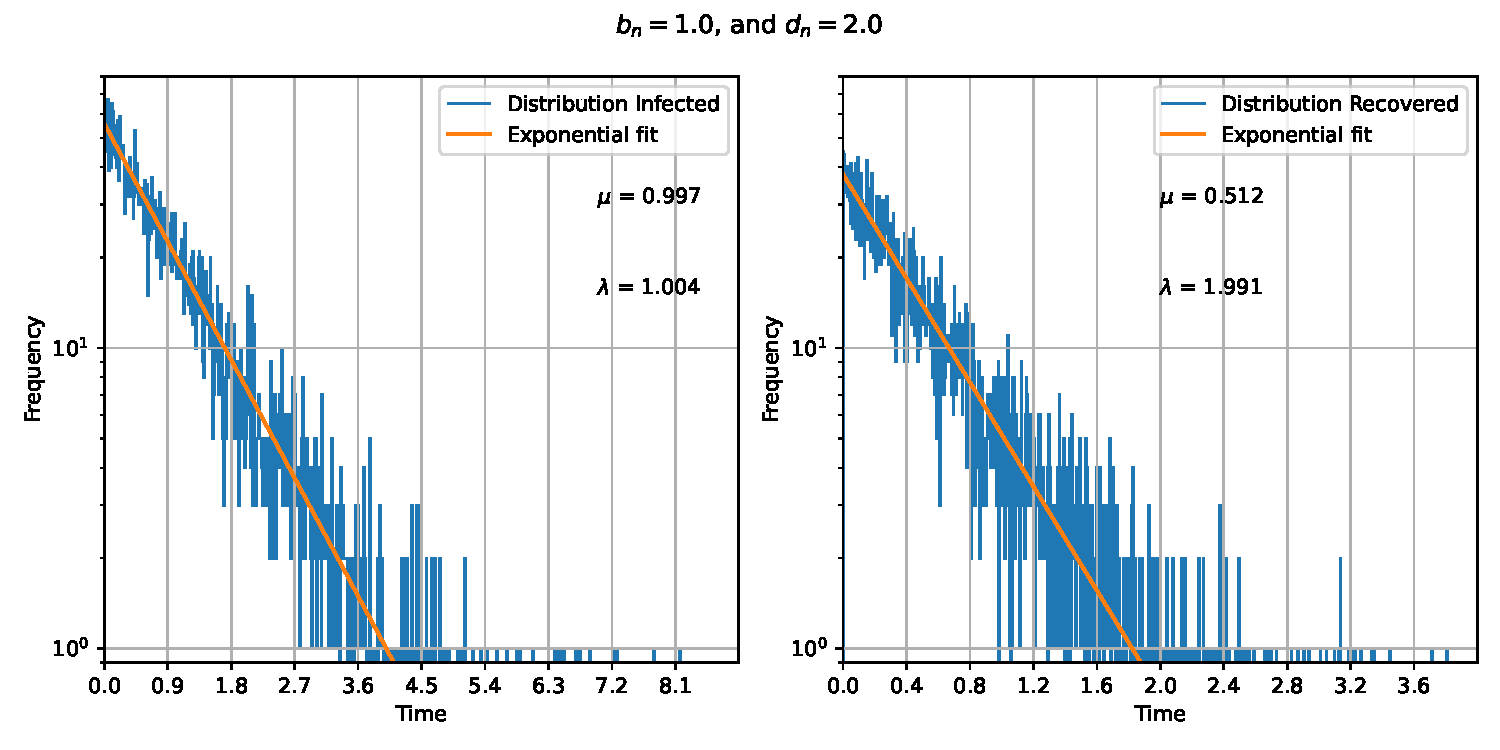
\includegraphics[width=0.95\textwidth]{figures/distribution_plot2.pdf}
	\end{center}
	\caption{In the left plot we can see the distribution for the infection time with a $b_n = 1.0$. We see that the fitted exponential distribution fits very well where we get a $\lambda = 1.0$ and a mean value of close to $\mu = \frac{1}{\lambda}$. In the left plot we have the distribution of the recovery time. Also here the exponential distribution fits well to the data and we get a $\lambda = d_n$ and a $\mu \approx \frac{1}{\lambda}$.}\label{fig:plot2}
\end{figure}

\begin{figure}[H]
	\begin{center}
		
\includegraphics[width=0.95\textwidth]{figures/distribution_plot3.pdf}
	\end{center}
	\caption{In the left plot we can see the distribution for the infection time with a $b_n = 10.0$. We see that the fitted exponential distribution fits very well where we get a $\lambda = 10.0$ and a mean value of close to $\mu = \frac{1}{\lambda}$. In the left plot we have the distribution of the recovery time. Also here the exponential distribution fits well to the data and we get a $\lambda = d_n$ and a $\mu \approx \frac{1}{\lambda}$.}\label{fig:plot3}
\end{figure}

From the samples we can clearly state that approximating the distributions with a exponential distribution works well and the mean value of the distribution is $1/\lambda$. This is is is a nice result as $\lambda$ is the mean rate of infections per time unit, which makes it natural that the inverse of this creates the mean time to every infection.

\subsection{d)}
In this section the stochastic simulation where supposed to be carried out and sampled for to create the distribution for the probability of a specific population while having the starting point in the deterministic stable point. The time to extinction is defined for the system as the average time for the population to go extinct and have the following relation:
\begin{equation}
	T_{ext} \sim e^{NS(0)}, \text{ where }S(0) = Log(r_0) - (1 - \frac{1}{r_0})
\end{equation}
To prevent $S(0)$ from getting to large we choose a appropriate values of $\alpha$ and $\beta$ which were decided to be $\alpha = 0.112$ and $\beta = 0.1$ with a total population of $N = 1000$. This also sets the $n_0 = I^*_2 \approx 107$. To analyze the quasi steady state distribution the time steps we recorded where $t_1<T_{ext}$, $t_2 \approx T_{ext}$ and $t_3 > T_{ext}$. To get a proper evaluation of $T_{ext}$ we sampled 5000 samples for 10 000 000 time steps and got $T_{ext} \approx 37125 $. Then we ran the simulation to collect the time samples for $t_1$, $t_2$ and $t_3$. The results can be found in figure \ref{fig:simulated results}.
\begin{figure}[H]
	\begin{center}
		
\includegraphics[width=0.99\textwidth]{figures/plot_dist_pn.pdf}
	\end{center}
	\caption{In this figure we see the results of the sampled simulations for 3 different time steps. For the first time the sampled distribution follow a gaussian distribution well with where you can see a heavier left tail and a lighter right tail. The plot in the middle with a time near the $T_{ext}$ is also close to the gaussian distribution but both the left and right wing has become weaker. In the final plot we can see that the whole distribution has become much lower and most of the sampled infections has become extinct.}\label{fig:simulated results}
\end{figure}
The gaussian distribution that we are comparing with in the plots have the following expression:
\begin{equation}
	\rho_0(I,t) \sim Ae^{-NS_0(I)} = Ae^{- \frac{(I-I^*_2)^2}{N/r_0}}
\end{equation}
where $S_0(I) = \frac{r_0}{2}(I/N - I^*_2/N) ^2$, which makes the mean value $\mu = I^*_2$ and variance $\sigma^2 = \frac{N}{r_0}$. We can see that for $t \leq T_{ext}$ the curve follow the gaussian form relatively well. In the earlier plot we can see a heavier left side and a lighter left side of the distribution, which is exactly what theory predicts. This heavier tail is kept for later times but as more at $t \approx T_{ext}$ the distribution is still relatively approximate the gaussian distribution. But for higher $t$ this approximation breaks down as more of the population reach the $I^*_1 = 0$.

\begin{verbatim}
import numpy as np
from scipy.optimize import curve_fit
import matplotlib.pyplot as plt


def exp_model(x, a, b):
    return a * np.exp(-b * x)


def check_probability(p: float) -> bool:
    rand = np.random.rand()
    if p > rand:
        return True
    else:
        return False


def draw_outcome(p_b: float, p_d: float) -> str:
    if check_probability(p_b + p_d):
        pb_probability = p_b / (p_b + p_d)
        if check_probability(pb_probability):
            return "new infection"
        else:
            return "new recovery"
    else:
        return "nothing happened"


def get_distribution(b: float, d: float, dt: float, total_samples: int):
    distribution_infections = []
    distribution_recovery = []
    samples = 0
    time = 0.0
    p_b = b * dt
    p_d = d * dt

    saved_infection = False
    saved_recovery = False
    while total_samples > samples:
        time += dt
        outcome = draw_outcome(p_b, p_d)
        if (outcome == "new infection") and not (saved_infection):
            distribution_infections.append(time)
            saved_infection = True
            samples += 1
        elif outcome == "new recovery" and not (saved_recovery):
            saved_recovery = True
            distribution_recovery.append(time)
            samples += 1

        if saved_infection and saved_recovery:
            time = 0.0
            saved_infection = False
            saved_recovery = False

        if samples % 100 == 0 and samples != 0:
            print(samples)
    distribution_infections = np.array(distribution_infections)
    distribution_recovery = np.array(distribution_recovery)

    np.save(f"infection_distribution3.npy", distribution_infections)
    np.save("recovery_distribution3.npy", distribution_recovery)


def plot_distribution(distr_inf, distr_rec: np.ndarray, file_name: str):
    fig, ax = plt.subplots(1, 2, figsize=(10, 5))
    hist_inf, bins_inf = np.histogram(distr_inf, bins=1000)
    hist_rec, bins_rec = np.histogram(distr_rec, bins=1000)
    t_inf = np.linspace(bins_inf[0], bins_inf[-1], 1000)
    t_rec = np.linspace(bins_rec[0], bins_rec[-1], 1000)

    params_inf, covariance_inf = curve_fit(exp_model, bins_inf[1:], hist_inf)
    params_rec, covariance_rec = curve_fit(exp_model, bins_rec[1:], hist_rec)
    a_inf, lambda_inf = params_inf
    a_rec, lambda_rec = params_rec

    mean_low_inf = np.average(bins_inf[:-1], weights=hist_inf)
    mean_high_inf = np.average(bins_inf[1:], weights=hist_inf)

    mean_inf = (mean_low_inf + mean_high_inf) / 2

    mean_low_rec = np.average(bins_rec[:-1], weights=hist_rec)
    mean_high_rec = np.average(bins_rec[1:], weights=hist_rec)
    mean_rec = (mean_low_rec + mean_high_rec) / 2

    ax[0].stairs(hist_inf, bins_inf, label="Distribution Infected")
    ax[0].plot(t_inf, exp_model(t_inf, a_inf, lambda_inf), label="Exponential fit")
    ax[0].set_xticks(np.arange(0, 1, 0.1))
    ax[0].set_yscale("log")
    ax[0].text(0.7, 15, rf"$\lambda$ = {lambda_inf:.3f}")
    ax[0].text(0.7, 30, rf"$\mu$ = {mean_inf:.3f}")
    ax[0].set_xlim(0, 1)
    ax[0].set_ylim(0.9, 80)
    ax[0].set_xlabel("Time")
    ax[0].set_ylabel("Frequency")
    ax[0].grid()
    ax[0].legend()

    ax[1].stairs(hist_rec, bins_rec, label="Distribution Recovered")
    ax[1].plot(t_rec, exp_model(t_rec, a_rec, lambda_rec), label="Exponential fit")
    ax[1].set_xticks(np.arange(0, 1, 0.1))
    ax[1].set_yscale("log")
    ax[1].text(0.7, 15, rf"$\lambda$ = {lambda_rec:.3f}")
    ax[1].text(0.7, 30, rf"$\mu$ = {mean_rec:.3f}")
    ax[1].set_xlim(0, 1)
    ax[1].set_ylim(0.9, 80)
    ax[1].set_xlabel("Time")
    ax[1].set_ylabel("Frequency")
    ax[1].grid()
    ax[1].legend()
    fig.suptitle(rf"$b_n = {lambda_inf:.1f}$, and $d_n = {lambda_rec:.1f}$")
    fig.tight_layout()
    fig.savefig(file_name)


def c():
    b = 10
    d = 5
    time_step = 1e-6
    total_samples = 10000
    # get_distribution(b, d, time_step, total_samples)
    infection_dis = np.load("infection_distribution3.npy")
    recovery_dis = np.load("recovery_distribution3.npy")

    plot_distribution(
        infection_dis, recovery_dis, "../report1/figures/distribution_plot3.pdf"
    )


def get_next_event(dist_infected: np.ndarray, dist_recovery: np.ndarray):
    rand_index_infected = np.random.randint(0, dist_infected.shape[0])
    rand_index_recovery = np.random.randint(0, dist_recovery.shape[0])

    time_infected = dist_infected[rand_index_infected]
    time_recovery = dist_infected[rand_index_recovery]
    if time_infected > time_recovery:
        event_type = "recovery"
        time = time_recovery
        return event_type, time
    else:
        event_type = "infection"
        time = time_infected
        return event_type, time


def print_calculations(alpha: float, beta: float, N: float):
    r_0 = alpha / beta
    s_0 = np.log(r_0) - (1 - 1 / r_0)
    t_ext = np.exp(N * s_0)
    I_star = N * (1 - 1 / r_0)
    print(f"T_exit = {t_ext}")
    print(f"I_star = {I_star}")


def run_simulation(
    samples: int,
    record_times: np.ndarray,
    starting_infected: int,
    total_population: int,
    alpha: float,
    beta: float,
    total_simulation_time: int,
):
    n = np.zeros(samples, dtype=int)
    n[:] = starting_infected
    time = np.zeros(samples)
    has_recorded = np.zeros((samples, 3), dtype=bool)
    t_exit = []
    saved_n = np.zeros((samples, 3))
    n_zero = n <= 0
    n_max = n >= total_population
    t_b = np.zeros_like(time)
    t_d = np.zeros_like(time)

    for i in range(total_simulation_time):
        if i % 1000 == 0:
            print(i)
        b_n = alpha * n * (1 - n / total_population)
        d_n = beta * n
        t_b[n_zero] = 1e5
        t_b[~n_zero] = np.random.exponential(1 / b_n[~n_zero])
        t_b[n_max] = 1e5

        t_d[n_zero] = 1e5
        t_d[~n_zero] = np.random.exponential(1 / d_n[~n_zero])

        t_b_smaller = (t_b - t_d) < 0
        t_d_smaller = (t_d - t_b) < 0

        time[t_d_smaller] += t_d[t_d_smaller]
        time[t_b_smaller] += t_b[t_b_smaller]

        n[t_b_smaller] += 1
        n[t_d_smaller] -= 1

        n_zero = n <= 0

        n_max = n == total_population

        to_save = (~has_recorded) & (
            (time[:, None] >= record_times[None, :]) | (n_zero[:, None])
        )
        saved_n[to_save] = np.broadcast_to(n[:, None], (n.shape[0], 3))[to_save]
        has_recorded[to_save] = True

    # assert has_recorded.all() == True
    print(np.mean(time[n_zero]))
    print(np.sum(n_zero) / samples)
    print(np.sum(has_recorded) / (samples * 3))

    return saved_n


def gaussian_func(x: np.ndarray, mean: float, variance: float):
    return (
        1
        / (np.sqrt(2 * np.pi * variance))
        * np.exp(-((x - mean) ** 2) / (2 * variance))
    )


def d():
    alpha = 0.112
    beta = 0.1
    N = 1000
    samples = 5000
    simulation_time = 10000000
    t_record = np.array([10000, 37125, 60000])

    print_calculations(alpha, beta, N)

    n_start = 107
    variance = N * beta / alpha
    n = run_simulation(samples, t_record, n_start, N, alpha, beta, simulation_time)
    fig, axes = plt.subplots(1, 3, figsize=(15, 5), sharey=True, sharex=True)
    for idx, ax in enumerate(axes):
        hist, bins = np.histogram(n[:, idx], bins=100, density=True)
        bin_min = bins[0]
        bin_max = bins[-1]
        x = np.linspace(bin_min, bin_max, 1000)

        ax.stairs(-np.log(hist), bins, label="sampled simulations")
        ax.plot(
            x, -np.log(gaussian_func(x, n_start, variance)), label="gaussian function"
        )

        ax.axvline(n_start, label=r"$I^*_2$", c="black")
        ax.set_title(rf" $t = {t_record[idx]}$")
        ax.set_xlabel(r"$n_t$")
        ax.set_ylabel(r"$-Log\left(p(n_t)\right)$")
        ax.legend()

    fig.tight_layout()
    fig.savefig("../report1/figures/plot_dist_pn.pdf")


def main():
    # c()
    d()
    # test()


if __name__ == "__main__":
    main()
\end{verbatim}

\end{document}
